\documentclass[a4paper,10pt]{article}
\usepackage[utf8]{inputenc}
\usepackage[T1]{fontenc}
\usepackage[sc]{mathpazo}
\usepackage[scaled=0.88]{helvet}
\usepackage{amsmath,amssymb,mathrsfs,stmaryrd}
\usepackage{microtype}
\usepackage[a4paper,top=1.5cm,bottom=1.5cm,left=1.4cm,right=1.4cm,headheight=12pt,headsep=0.4cm,footskip=0.7cm]{geometry}
\usepackage{xcolor}
\definecolor{Ink}{HTML}{1C2533}\definecolor{Bleu}{HTML}{1F3A5F}\definecolor{BleuMoyen}{HTML}{4A6A8F}
\definecolor{BleuClair}{HTML}{9DB2C9}\definecolor{Fond}{HTML}{F2F4F7}\definecolor{Ocre}{HTML}{B07A26}
\definecolor{Brique}{HTML}{A23B2A}\definecolor{Gris}{HTML}{5E6672}\definecolor{Filet}{HTML}{C5CCD6}
\usepackage{multicol,enumitem,booktabs,array,needspace}
\usepackage[most]{tcolorbox}
\usepackage{tikz,pgfplots}
\pgfplotsset{compat=1.17,trig format plots=rad}
\usetikzlibrary{arrows.meta,positioning,shapes.geometric}
\usepackage{fancyhdr}
\usepackage[colorlinks=true,linkcolor=Bleu,bookmarksopen=true,bookmarksopenlevel=0]{hyperref}

\setlength{\parindent}{0pt}\setlength{\parskip}{0.25em}
\setlength{\columnsep}{0.55cm}\setlength{\columnseprule}{0.3pt}\renewcommand{\columnseprulecolor}{\color{Filet}}
\setlist{itemsep=0.05em,topsep=0.15em,parsep=0pt,leftmargin=1.1em}
\setlist[itemize]{label=\textcolor{BleuMoyen}{\scriptsize\textbullet}}
\setlist[enumerate]{label=\textsf{\scriptsize\color{Bleu}\arabic*.},leftmargin=1.3em}
\linespread{1.02}

\newcommand{\K}{\mathbb{K}}\newcommand{\R}{\mathbb{R}}\newcommand{\C}{\mathbb{C}}\newcommand{\Z}{\mathbb{Z}}
\newcommand{\Mn}[1]{\mathcal{M}_{n}(#1)}\newcommand{\rg}{\operatorname{rg}}\newcommand{\vect}{\operatorname{Vect}}
\newcommand{\Mat}{\operatorname{Mat}}\newcommand{\Id}{\operatorname{Id}}\newcommand{\com}{\operatorname{com}}
\newcommand{\vv}[1]{\overrightarrow{#1}}\newcommand{\ve}[1]{\vec{#1}}
\newcommand{\dt}[1]{\left|\begin{matrix}#1\end{matrix}\right|}
\newcommand{\HP}{{\sffamily\bfseries\scriptsize\textcolor{Brique}{[HP]}}}
\newcommand{\livre}[1]{{\sffamily\scriptsize\color{Gris}[#1]}}

% ---------- titres ----------
\newcommand{\chapitre}[2]{\clearpage\phantomsection\pdfbookmark[0]{#1 --- #2}{chap#1}\markboth{#1 --- #2}{}%
  \noindent\colorbox{Bleu}{\parbox{\dimexpr\linewidth-2\fboxsep}{\color{white}\sffamily\bfseries\Large\strut #1\quad
  {\normalsize\mdseries #2}}}\par\vspace{0.4em}}
\newcommand{\notion}[1]{\par\needspace{9\baselineskip}\vspace{0.5em}\phantomsection\pdfbookmark[1]{#1}{\detokenize{#1}}\noindent{\sffamily\bfseries\color{Bleu}\large #1}\par\nobreak
  \noindent{\color{Ocre}\rule{\linewidth}{0.8pt}}\par\nobreak\vspace{0.1em}}
\newcommand{\sous}[1]{\par\needspace{6\baselineskip}\vspace{0.25em}\noindent{\sffamily\bfseries\small\color{BleuMoyen}#1}\par\nobreak}

% ---------- encadrés ----------
\tcbset{base/.style={enhanced,arc=0pt,boxrule=0pt,left=4pt,right=3pt,top=2pt,bottom=2pt,before skip=0.35em,after skip=0.35em,
  fontupper=\small}}
\newtcolorbox{DEF}[1][]{base,colback=white,borderline west={1.4pt}{0pt}{Bleu},
  before upper={{\sffamily\bfseries\scriptsize\color{Bleu}DÉFINITION\ifx\relax#1\relax\else\ --- #1\fi}\par}}
\newtcolorbox{PROP}[1][]{base,colback=Fond,borderline west={2pt}{0pt}{Bleu},
  before upper={{\sffamily\bfseries\scriptsize\color{Bleu}\ifx\relax#1\relax PROPRIÉTÉ\else #1\fi}\par}}
\newtcolorbox{FORM}[1][]{base,colback=white,colframe=BleuMoyen,boxrule=0.5pt,
  before upper={{\sffamily\bfseries\scriptsize\color{BleuMoyen}\ifx\relax#1\relax FORMULES\else #1\fi}\par}}
\newtcolorbox{METH}[1]{base,colback=white,borderline north={0.8pt}{0pt}{Bleu},borderline south={0.8pt}{0pt}{Bleu},
  before upper={{\sffamily\bfseries\scriptsize\colorbox{Bleu}{\color{white}MÉTHODE}\ \color{Bleu}#1}\par\smallskip}}
\newtcolorbox{PIEGE}{base,colback=Brique!5,borderline west={1.4pt}{0pt}{Brique},
  before upper={{\sffamily\bfseries\scriptsize\color{Brique}PIÈGES}\par}}
\newtcolorbox{ASTU}{base,colback=Ocre!7,borderline west={1.4pt}{0pt}{Ocre},
  before upper={{\sffamily\bfseries\scriptsize\color{Ocre}ASTUCES}\par}}
\newtcolorbox{REFL}{base,colback=Bleu!4,borderline west={2pt}{0pt}{BleuMoyen},
  before upper={{\sffamily\bfseries\scriptsize\color{BleuMoyen}RÉFLEXES AVANT DE RENDRE}\par}}
\tikzset{q/.style={draw=Bleu,fill=Fond,rounded corners=2pt,font=\scriptsize\sffamily,align=center,inner sep=3pt},
  oui/.style={draw=Bleu,fill=Bleu,text=white,rounded corners=2pt,font=\scriptsize\sffamily\bfseries,align=center,inner sep=3pt},
  non/.style={draw=Brique,fill=Brique!8,text=Brique,rounded corners=2pt,font=\scriptsize\sffamily\bfseries,align=center,inner sep=3pt},
  fl/.style={-{Stealth[length=4pt]},Gris,thin},lab/.style={font=\tiny\sffamily,text=Gris}}
\newtcolorbox{HPBOX}{base,colback=white,borderline west={1.4pt}{0pt}{Brique},
  before upper={{\sffamily\bfseries\scriptsize\color{Brique}HORS PROGRAMME}\par}}

\pagestyle{fancy}\fancyhf{}
\fancyhead[L]{\scriptsize\sffamily\color{Gris}\leftmark}
\fancyhead[R]{\scriptsize\sffamily\scshape\color{Gris}Le Collé PT --- fiche Séries entières}
\fancyfoot[C]{\scriptsize\sffamily\thepage}
\renewcommand{\headrulewidth}{0.3pt}

\pgfplotsset{mini/.style={axis lines=middle,axis line style={Filet},xtick=\empty,ytick=\empty,width=3.2cm,height=3.2cm,
  xmin=-1.15,xmax=1.15,ymin=-1.15,ymax=1.15,title style={font=\scriptsize\sffamily,yshift=-0.15cm},samples=80}}


\newcommand{\Ker}{\operatorname{Ker}}\renewcommand{\Im}{\operatorname{Im}}\newcommand{\tr}{\operatorname{tr}}\newcommand{\Sp}{\operatorname{Sp}}
\newcommand{\GLn}[1]{\mathrm{GL}_n(#1)}
\hypersetup{pdftitle={Le Collé — fiche de référence : séries numériques}}
\providecommand{\ch}{\operatorname{ch}}\providecommand{\sh}{\operatorname{sh}}
\begin{document}
\thispagestyle{empty}
\noindent\colorbox{Bleu}{\parbox{\dimexpr\linewidth-2\fboxsep}{\vspace{0.4em}
{\color{white}\sffamily\scriptsize\textls[200]{LE COLLÉ\ \ ·\ \ MATHÉMATIQUES PT\ \ ·\ \ CHAPITRE 8}}\par\smallskip
{\color{white}\sffamily\bfseries\LARGE Fiche de référence --- Séries entières}\par\smallskip
{\color{white!85!Bleu}\sffamily série de Taylor, rayon de convergence, fonction somme, développements usuels, méthodes, quelle méthode ?}\vspace{0.4em}}}

\vspace{0.6em}
{\small Le livret sert à apprendre, la présentation à comprendre, cette fiche à réviser : tout le cours du chapitre (définitions, théorèmes, formules, méthodes, pièges), avec les mêmes numéros de parties et les mêmes notations que le livret ; \livre{th.~1.12} y renvoie. $\sum a_nz^n$ série entière, $R$ son rayon ; DSE : développement en série entière.}

\vspace{0.4em}
{\small\sffamily\noindent\begin{tabular}{@{}p{0.6\linewidth}@{}}
1.1 Série de Taylor d'une fonction \dotfill\pageref{n11}\\
1.2 Séries entières, rayon de convergence \dotfill\pageref{n12}\\
1.3 Calcul du rayon de convergence \dotfill\pageref{n13}\\
1.4 Fonction somme d'une série entière réelle \dotfill\pageref{n14}\\
1.5 Fonctions développables en série entière \dotfill\pageref{n15}\\
1.6 Développer une fonction en série entière \dotfill\pageref{n16}\\
1.7 Quelle méthode ? Synthèse \dotfill\pageref{n17}\\
\end{tabular}}

\vspace{0.6em}
\pdfbookmark[0]{Chapitre 8 --- Séries entières}{chap8}\markboth{Chapitre 8 --- Séries entières}{}
\begin{multicols}{2}\raggedcolumns
% ======================================================================
\notion{1.1 Série de Taylor d'une fonction}\label{n11}

\begin{PROP}[TAYLOR AVEC RESTE INTÉGRAL \livre{th.~1.1}]
$f$ de classe $\mathcal C^{n+1}$ sur $I\ni0$ :\
$\displaystyle f(x)=\sum_{k=0}^n\frac{f^{(k)}(0)}{k!}x^k+\int_0^x\frac{(x-t)^n}{n!}f^{(n+1)}(t)\,dt$.\\
Taylor-Lagrange : $|R_n(x)|\leq M\frac{|x|^{n+1}}{(n+1)!}$ si $|f^{(n+1)}|\leq M$ \livre{cor.~1.2}.
\end{PROP}

\begin{DEF}[SÉRIE DE TAYLOR \livre{déf.~1.3}]
$\sum\frac{f^{(n)}(0)}{n!}x^n$ ; sa somme vaut $f(x)$ $\iff R_n(x)\to0$.
\end{DEF}

\begin{FORM}[FAMILLE EXPONENTIELLE, $x\in\R$ \livre{th.~1.4, 1.6}]
$e^x=\sum\frac{x^n}{n!}$ ;\quad $\ch x=\sum\frac{x^{2n}}{(2n)!}$,\ $\sh x=\sum\frac{x^{2n+1}}{(2n+1)!}$ ;\\
$\cos x=\sum\frac{(-1)^nx^{2n}}{(2n)!}$,\ $\sin x=\sum\frac{(-1)^nx^{2n+1}}{(2n+1)!}$.
\end{FORM}

\begin{METH}{Somme avec des factorielles \livre{méth.~1.1}}
Factoriser la puissance en trop, changer d'indice ; $P(n)$ sur la base $n(n-1)$, $n$, $1$ ; $x=t^2$ ou $x=-t^2$ devant $(2n)!$.
Ex. : $\sum_{n\geq0}\frac{n^2}{n!}=2e$.
\end{METH}

\begin{PIEGE}
$\mathcal C^\infty$ ne suffit pas : $e^{-1/x^2}$ a une série de Taylor nulle. Toujours étudier le reste.
\end{PIEGE}

% ======================================================================
\notion{1.2 Séries entières, rayon de convergence}\label{n12}

\begin{PROP}[LEMME D'ABEL \livre{prop.~1.10}]
$(a_nz_0^n)$ bornée et $|z|<|z_0|$ $\Rightarrow$ $\sum a_nz^n$ converge absolument.
\end{PROP}

\begin{DEF}[RAYON \livre{déf.~1.11}]
$R=\sup\{r\geq0:(a_nr^n)\text{ bornée}\}\in[0,+\infty]$.
\end{DEF}

\begin{PROP}[\livre{th.~1.12}]
$|z|<R$ : CV absolue.\quad $|z|>R$ : DV grossière.\quad $|z|=R$ : on ne sait pas.
\end{PROP}

\begin{PROP}[ENCADRER \livre{prop.~1.15}]
$\sum a_nz_0^n$ CV $\Rightarrow R\geq|z_0|$ ;\ DV $\Rightarrow R\leq|z_0|$ ;\ CV non absolue $\Rightarrow R=|z_0|$.
\end{PROP}

% ======================================================================
\notion{1.3 Calcul du rayon de convergence}\label{n13}

\begin{PROP}[COMPARAISON, ÉQUIVALENTS \livre{prop.~1.17, 1.18}]
$|a_n|\leq|b_n|$ (ou $a_n=O(b_n)$) $\Rightarrow R_a\geq R_b$.\quad $|a_n|\sim|b_n|\Rightarrow R_a=R_b$.\\
$\sum n^\alpha a_nz^n$ et $\sum a_nz^n$ : même rayon ; $\sum n^\alpha z^n$ : $R=1$ \livre{prop.~1.21}.
\end{PROP}

\begin{METH}{D'Alembert \livre{méth.~1.2}}
Sur la série \emph{numérique} $\sum|a_nz^n|$ : $\frac{|a_{n+1}|}{|a_n|}|z|\to L|z|$, donc $R=\frac1L$.\\
Série lacunaire ($z^{2n}$) : quotient des termes présents.
\end{METH}

\begin{PROP}[SOMME, PRODUIT DE CAUCHY \livre{prop.~1.22, th.~1.23}]
$R_{a+b}\geq\min(R_a,R_b)$, égalité si $R_a\neq R_b$.\\
$c_n=\sum_{k=0}^na_kb_{n-k}$ : $R\geq\min(R_a,R_b)$ et $\sum c_nz^n=\sum a_nz^n\cdot\sum b_nz^n$.
\end{PROP}

\begin{FORM}[RAYONS DE RÉFÉRENCE]
$\sum z^n$, $\sum\frac{z^n}n$, $\sum n^\alpha z^n$ : $1$ ;\ $\sum\frac{z^n}{n!}$ : $+\infty$ ;\ $\sum n!z^n$ : $0$ ;\ $\sum\lambda^nz^n$ : $\frac1{|\lambda|}$.
\end{FORM}

\begin{PIEGE}
D'Alembert sur les $a_n$ quand une infinité sont nuls. Conclure au bord à partir de $R$.
\end{PIEGE}

% ======================================================================
\notion{1.4 Fonction somme d'une série entière réelle}\label{n14}

\begin{PROP}[{RÉGULARITÉ SUR $]-R,R[$} \livre{th.~1.27, 1.29, cor.~1.30}]
$f(x)=\sum a_nx^n$ est continue, $\mathcal C^\infty$ ; $f'(x)=\sum_{n\geq1}na_nx^{n-1}$ (même $R$) ;\ $a_p=\frac{f^{(p)}(0)}{p!}$.
\end{PROP}

\begin{PROP}[INTÉGRATION \livre{th.~1.31}]
$\displaystyle\int_0^x\sum a_nt^n\,dt=\sum\frac{a_n}{n+1}x^{n+1}$ (même $R$).
\end{PROP}

\begin{PROP}[AU BORD \livre{prop.~1.28}, admis]
Si $\sum a_nR^n$ converge : $\sum a_nR^n=\lim_{x\to R^-}f(x)$. Ex. : $\sum_{n\geq1}\frac{(-1)^n}n=-\ln2$.
\end{PROP}

\begin{METH}{Calculer une somme \livre{méth.~1.4}}
1. Le rayon. 2. $P(n)x^n$ : dériver $\frac1{1-x}$, base $(n+1)(n+2)$, $n+1$, $1$. 3. $\frac{x^n}{n+k}$, fraction : intégrer, éléments simples.
4. $n!$ : famille exponentielle. 5. Contrôler en $0$.
\end{METH}

\begin{FORM}[À PARTIR DE $\frac1{1-x}$, $|x|<1$]
$\sum_{n\geq1}nx^n=\frac x{(1-x)^2}$ ;\ $\sum(n+1)x^n=\frac1{(1-x)^2}$ ;\ $\sum n^2x^n=\frac{x(1+x)}{(1-x)^3}$ ;\ $\sum_{n\geq1}\frac{x^n}n=-\ln(1-x)$.
\end{FORM}

% ======================================================================
\notion{1.5 Fonctions développables en série entière}\label{n15}

\begin{PROP}[DSE = SÉRIE DE TAYLOR \livre{th.~1.35}]
$f$ DSE sur $]-r,r[$ $\Rightarrow$ $f$ est $\mathcal C^\infty$ et $f(x)=\sum\frac{f^{(n)}(0)}{n!}x^n$ : DSE \emph{unique}.
Paire : puissances paires ; impaire : impaires \livre{prop.~1.36}.
\end{PROP}

\begin{FORM}[DSE USUELS \livre{tab.~1.1}]
$R=+\infty$ : $e^x$, $\ch$, $\sh$, $\cos$, $\sin$ (§1.1).\\[2pt]
$R=1$ : $\frac1{1-x}=\sum x^n$,\ $\frac1{1+x}=\sum(-1)^nx^n$,\\
$\ln(1+x)=\sum_{n\geq1}\frac{(-1)^{n+1}}nx^n$,\ $\ln(1-x)=-\sum_{n\geq1}\frac{x^n}n$,\\
$\arctan x=\sum\frac{(-1)^n}{2n+1}x^{2n+1}$,\\
$(1+x)^\alpha=1+\sum_{n\geq1}\frac{\alpha(\alpha-1)\cdots(\alpha-n+1)}{n!}x^n$.\\[2pt]
$\C$ : $e^z=\sum\frac{z^n}{n!}$, $e^{z+z'}=e^ze^{z'}$ \livre{th.~1.40}.
\end{FORM}

% ======================================================================
\notion{1.6 Développer une fonction en série entière}\label{n16}

\begin{METH}{Opérations \livre{méth.~1.5}}
Substitution ($-x$, $x^2$, $-x^2$, $ax$) ; combinaison ; produit de Cauchy ; dérivation, intégration (+ $f(0)$) ;
éléments simples : $\frac a{x-\lambda}=-\frac a\lambda\cdot\frac1{1-x/\lambda}$, $|x|<|\lambda|$.
\end{METH}

\begin{METH}{Équation différentielle \livre{méth.~1.6}}
1. Équation vérifiée par $f$ + conditions initiales. 2. Analyse : $y=\sum a_nx^n$, réindexer en $x^n$, unicité $\Rightarrow$ récurrence.
3. Résoudre. 4. Synthèse : rayon $R$. 5. Unicité de Cauchy (coefficient dominant non nul).
\end{METH}

\begin{PIEGE}
Préciser l'intervalle : $\frac1{1+x^2}=\sum(-1)^nx^{2n}$ seulement pour $|x|<1$. Indice de départ qui change en dérivant.
\end{PIEGE}

% ======================================================================
\notion{1.7 Quelle méthode ? Synthèse}\label{n17}

\sous{Rayon de $\sum a_nz^n$ : l'arbre de décision}
\begin{center}
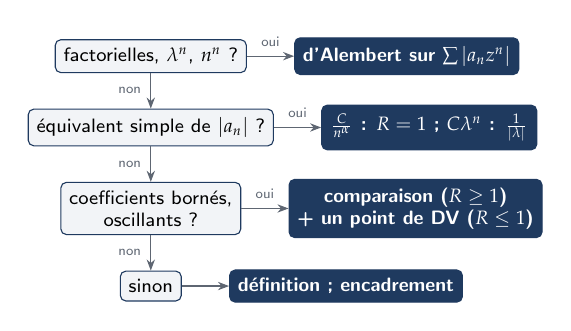
\begin{tikzpicture}[node distance=4.5mm and 6mm]
\node[q] (a) {factorielles, $\lambda^n$, $n^n$ ?};
\node[oui,right=of a] (a2) {d'Alembert sur $\sum|a_nz^n|$};
\node[q,below=of a] (b) {équivalent simple de $|a_n|$ ?};
\node[oui,right=of b] (b2) {$\frac C{n^\alpha}$ : $R=1$ ;\ $C\lambda^n$ : $\frac1{|\lambda|}$};
\node[q,below=of b] (c) {coefficients bornés,\\oscillants ?};
\node[oui,right=of c] (c2) {comparaison ($R\geq1$)\\+ un point de DV ($R\leq1$)};
\node[q,below=of c] (d) {sinon};
\node[oui,right=of d] (d2) {définition ; encadrement};
\draw[fl] (a)--node[lab,above]{oui}(a2); \draw[fl] (a)--node[lab,left]{non}(b);
\draw[fl] (b)--node[lab,above]{oui}(b2); \draw[fl] (b)--node[lab,left]{non}(c);
\draw[fl] (c)--node[lab,above]{oui}(c2); \draw[fl] (c)--node[lab,left]{non}(d);
\draw[fl] (d)--(d2);
\end{tikzpicture}
\end{center}

\sous{Je vois\dots\ je fais\dots}
{\small\renewcommand{\arraystretch}{1.16}
\begin{tabular}{@{}>{\raggedright\arraybackslash}p{0.36\linewidth}>{\raggedright\arraybackslash}p{0.58\linewidth}@{}}
\toprule
\textsf{\scriptsize Question} & \textsf{\scriptsize Méthode}\\\midrule
nature en $x=\pm R$ & séries numériques : Riemann, alternée, divergence grossière\\
somme, $P(n)x^n$ & dériver $\frac1{1-x}$\\
somme, $\frac{x^n}{n+k}$, fraction & intégrer ; éléments simples\\
somme, $\frac{\cdots}{n!}$ & famille exponentielle\\
somme numérique $\sum a_n$ & $f(\pm1)$ et continuité au bord\\
DSE d'une fonction & substitution, opérations, dériver, intégrer\\
DSE « compliqué » & équation différentielle\\
$f^{(p)}(0)$ & $p!\,a_p$\\
solutions DSE d'une équation & récurrence sur $a_n$, puis rayon\\
\bottomrule
\end{tabular}}

\begin{PIEGE}
Tout peut arriver en $|z|=R$. Les théorèmes de dérivation et d'intégration valent sur l'intervalle \emph{ouvert}. Oublier
$F(0)$ en intégrant. Un DSE sans intervalle n'a pas de sens.
\end{PIEGE}

\begin{REFL}
Donner le rayon avant toute somme. Vérifier les premiers termes (en $x=0$, coefficient de $x$). Dire sur quel intervalle
l'égalité est valable. Après un DSE par équation différentielle : citer l'unicité de Cauchy.
\end{REFL}
\end{multicols}
\end{document}
